%%%%%%%%%%%%%%%%%%%%% PACKAGE IMPORTS %%%%%%%%%%%%%%%%%%%%%
\documentclass{article}
\usepackage{import}
\subimport*{./}{macro}

\usepackage{amsmath, amsfonts, amsthm, amssymb}
\usepackage{lmodern}
\usepackage{microtype}
\usepackage{fullpage}       
\usepackage{changepage}
\usepackage{hyperref}
\usepackage{blindtext}
\hypersetup{
    colorlinks=true,
    linkcolor=blue,
    filecolor=magenta,      
    urlcolor=blue,
    pdftitle={Overleaf Example},
    pdfpagemode=FullScreen,
    }
\urlstyle{same}

\newenvironment{level}%
{\addtolength{\itemindent}{2em}}%
{\addtolength{\itemindent}{-2em}}

\usepackage{amsmath,amsthm,amssymb}

\usepackage[nooldvoltagedirection]{circuitikz}
\usetikzlibrary{decorations,arrows,shapes}

\usepackage{datetime}
\usepackage{etoolbox}
\usepackage{enumerate}
\usepackage{enumitem}
\usepackage{listings}
\usepackage{array}
\usepackage{varwidth}
\usepackage{tcolorbox}
\usepackage{amsmath}
\usepackage{circuitikz}
\usepackage{verbatim}
\usepackage[linguistics]{forest}
\usepackage{listings}
\usepackage{xcolor}
\renewcommand{\rmdefault}{cmss}


\newcommand\doubleplus{+\kern-1.3ex+\kern0.8ex}
\newcommand\mdoubleplus{\ensuremath{\mathbin{+\mkern-10mu+}}}

\definecolor{codegreen}{rgb}{0,0.6,0}
\definecolor{codegray}{rgb}{0.5,0.5,0.5}
\definecolor{codepurple}{rgb}{0.58,0,0.82}
\definecolor{backcolour}{rgb}{0.95,0.95,0.92}

\lstdefinestyle{mystyle}{
    language=Python,
    basicstyle=\ttfamily\small,
    keywordstyle=\color{blue},
    stringstyle=\color{red},
    commentstyle=\color{green},
    morecomment=[l][\color{magenta}]{\#},
    backgroundcolor=\color{backcolour},   
    breakatwhitespace=false,         
    breaklines=true,                 
    captionpos=b,                    
    keepspaces=true,                 
    numbers=left,                    
    numbersep=5pt,                  
    showspaces=false,                
    showstringspaces=false,
    showtabs=false,                  
    tabsize=2
}

\lstset{style=mystyle}
\setlength{\parindent}{0pt}
\setlength{\parskip}{5pt plus 1pt}

\providetoggle{questionnumbers}
\settoggle{questionnumbers}{true}
\newcommand{\noquestionnumbers}{
    \settoggle{questionnumbers}{false}
}

\newcounter{questionCounter}
\newenvironment{question}[2][\arabic{questionCounter}]{%
    \ifnum\value{questionCounter}=0 \else {\newpage}\fi%
    \setcounter{partCounter}{0}%
    \vspace{.25in} \hrule \vspace{0.5em}%
    \noindent{\bf \iftoggle{questionnumbers}{Question #1: }{}#2}%
    \addtocounter{questionCounter}{1}%
    \vspace{0.8em} \hrule \vspace{.10in}%
}

\newcounter{partCounter}[questionCounter]
\renewenvironment{part}[1][\alph{partCounter}]{%
    \addtocounter{partCounter}{1}%
    \vspace{.10in}%
    \begin{indented}%
       {\bf (#1)} %
}{\end{indented}}

\def\indented#1{\list{}{}\item[]}
\let\indented=\endlist
\def\show#1{\ifdefempty{#1}{}{#1\\}}
\def\IMP{\longrightarrow}
\def\AND{\wedge}
\def\OR{\vee}
\def\BI{\leftrightarrow}
\def\DIFF{\setminus}
\def\SUB{\subseteq}


\newcolumntype{C}{>{\centering\arraybackslash}m{1.5cm}}
\renewcommand\qedsymbol{$\blacksquare$}
\newtcolorbox{answer}
{
  colback   = green!5!white,    % Background colorucyitc,
  colframe  = green!75!black,   % Outline color
  box align = center,           % Align box on text line
  varwidth upper,               % Enables multi line input
  hbox                          % Bounds box to text width
}

\newcommand{\myhwname}{CSE 446 Homework 0}
\newcommand{\myname}{Sebastian Liu}
\newcommand{\myemail}{ll57@cs.washington.edu}
\newcommand{\mysection}{AB}
\newcommand{\dollararrow}{\stackrel{\$}{\leftarrow}}
%%%%%%%%%%%%%%%%%%%%%%%%%%%%%%%%%%%%%%%%%%%%%%%%%%%%%%%%%%%

%%%%%%%%%%%%%%%%%%% Document Options %%%%%%%%%%%%%%%%%%%%%%
\noquestionnumbers
%%%%%%%%%%%%%%%%%%%%%%%%%%%%%%%%%%%%%%%%%%%%%%%%%%%%%%%%%%%

%%%%%%%%%%%%%%%%%%%%%%%% WORK BELOW %%%%%%%%%%%%%%%%%%%%%%%%
\begin{document}

\begin{center}
    \textbf{Homework 0} \bigskip
\end{center}

%%%%%%%%%%%%%%%%%%%%%%%% Task 1 %%%%%%%%%%%%%%%%%%%%%%%%M
\begin{question}{A1. (2 points)}
    \begin{part}
       \begin{answer}
           Let $X$ be the event that I test positive for the disease and $Y$ be the event that I have the disease. \\
           We are given:
             \begin{itemize}
                \item $\Prob{X | Y} = \frac{99}{100}$ 
                \item $\Prob{X^C | Y^C} = \frac{99}{100} $
                \item $\Prob{Y} = \frac{1}{10,000}$
             \end{itemize}
            Our goal is to find the probability that I have the disease given that I tested positive (i.e. $\Prob{Y | X}$). \\
            We can use Bayes' Theorem:
            \begin{align*}
                \Prob{Y | X} & = \frac{\Prob{X | Y} \cdot \Prob{Y}}{\Prob{X}} \\
                & = \frac{\Prob{X | Y} \cdot \Prob{Y}}{\Prob{X | Y} \cdot \Prob{Y} + \Prob{X | Y^C} \cdot \Prob{Y^C}} \tag{Law of Total Probability on $\Prob{X}$}\\
                & = \frac{\Prob{X | Y} \cdot \Prob{Y}}{\Prob{X | Y} \cdot \Prob{Y} + (1 - \Prob{X^C | Y^C}) \cdot (1 - \Prob{Y})}  \tag{Complement Rule} \\
                & = \frac{\frac{99}{100} \cdot \frac{1}{10,000}}{\frac{99}{100} \cdot \frac{1}{10,000} + (1 - \frac{99}{100}) \cdot (1 - \frac{1}{10,000})} \tag{plugging in given values} \\
                & = \frac{99}{10098} \\
                & \approx 0.0098
            \end{align*}
            Therefore, the probability that I actually have the disease is $\boxed{\frac{99}{10098} \approx 0.0098}$.
        \end{answer}
    \end{part}
\end{question}

%%%%%%%%%%%%%%%%%%%%%%%% Task 2 %%%%%%%%%%%%%%%%%%%%%%%%
\begin{question}{A2. (2 points)}
    \begin{part}
        \begin{answer}
           \begin{align*}
                \Cov{X}{Y} &= \E{(X - \E{X})(Y - \E{Y})} \tag{definition of covariance} \\
                &= \E{XY - X\E{Y} - Y\E{X} + \E{X}\E{Y}} \\
                &= \E{XY} - \E{X}\E{Y} - \E{Y}\E{X} + \E{X}\E{Y} \tag{linearity of expectation} \\
                &= \E{XY} - \E{X}\E{Y} \\
                &= (\sum \limits_{x \in \Omega_X} \sum \limits_{y \in \Omega_Y} xy \cdot \Prob{X = x, Y = y}) - \E{X}\E{Y} \tag{definition of expectation} \\
                &= (\sum \limits_{x \in \Omega_X} x \cdot (\sum \limits_{y \in \Omega_Y} y \cdot \Prob{Y | X = x}) \cdot \Prob{X = x}) - \E{X} \E{Y} \\
                &= (\sum \limits_{x \in \Omega_X} x \cdot \E{Y | X = x} \cdot \Prob{X = x}) - \E{X} \E{Y} \tag{definition of conditional expectation} \\
                &= (\sum \limits_{x \in \Omega_X} x^2 \cdot \Prob{X = x}) - \E{X} \E{Y} \tag{Since $\E{Y | X = x} = x$} \\
                &= \E{X^2} - \E{X} \E{Y} \tag{definition of expectation} \\
                &= \E{X^2} - \E{X} \cdot \sum \limits_{x \in \Omega_X} \E{Y | X = x} \cdot \Prob{X = x} \tag{Law of Total Expectation} \\
                &= \E{X^2} - \E{X} \cdot \sum \limits_{x \in \Omega_X} x \cdot \Prob{X = x}  \tag{Since $\E{Y | X = x} = x$} \\
                &= \E{X^2} - \E{X}^2 \tag{definition of expectation} \\
                &= \E{X^2} - 2\E{X}^2 + \E{X}^2 \\
                &= \E{X^2 - 2X\E{X} + \E{X}^2} \tag{linearaity of expectation} \\
                &= \E{(X - \E{X})^2} \\
           \end{align*}
         \end{answer}
     \end{part}

     \begin{part}
        \begin{answer}
            \begin{align*}
                \Cov{X}{Y} &= \E{(X - \E{X})(Y - \E{Y})} \tag{definition of covariance} \\
                &= \E{XY - X\E{Y} - Y\E{X} + \E{X}\E{Y}} \\
                &= \E{XY} - \E{X}\E{Y} - \E{Y}\E{X} + \E{X}\E{Y} \tag{linearity of expectation} \\
                &= \E{XY} - \E{X}\E{Y} \\
                &= \E{X}\E{Y} - \E{X}\E{Y} \tag{since $X$ and $Y$ are independent} \\
                &= 0
           \end{align*}
         \end{answer}
     \end{part}

\end{question}

%%%%%%%%%%%%%%%%%%%%%%%% Task 3 %%%%%%%%%%%%%%%%%%%%%%%%
\begin{question}{A3. (2 points)} 
    \begin{part}
        \begin{answer}
            \begin{align*}
                h(z) \diff z &= \Prob{z \leq Z \leq z + \diff z} \tag{Probability of $Z = z$ (continuous)} \\
                \Rightarrow h(z) \diff z &= \Prob{z \leq X + Y \leq z + \diff z} \tag{Since $Z = X + Y$} \\
                \Rightarrow h(z) \diff z &= \int_{-\infty}^{\infty}  f(x) \cdot \Prob{z - x \leq Y \leq z - x + \diff z | X = x}  \diff x \tag{Law of Total Probability (continuous)} \\
                \Rightarrow h(z) \diff z &= \int_{-\infty}^{\infty}  f(x) \cdot \Prob{z - x \leq Y \leq z - x + \diff z} \diff x \tag{Since $X$ and $Y$ are independent} \\
                \Rightarrow h(z) \diff z &= \int_{-\infty}^{\infty}  f(x) \cdot g(z - x) \diff x \diff z \tag{Def. PDF} \\
                \Rightarrow h(z) &= \int_{-\infty}^{\infty}  f(x) \cdot g(z - x) \diff x \tag{$\diff z$ cancels out}
            \end{align*}
        \end{answer}
     \end{part}

     \begin{part}
        \begin{answer}
            When $ 0 \le z \le 1$, since $z = x + y$, we know $0 \le x \le z$.\\
            Since $X$ and $Y$ are uniform on $[0, 1]$, we have: $$h(z) = \int_{-\infty}^{\infty}  f(x) \cdot g(z - x) \diff x  = 
            \int_{0}^{z}  1 \cdot 1 \diff x = z$$
            When $1 < z \le 2$, since $z = x + y$, we know $z - 1 \le x \le 1$.\\
            Since $X$ and $Y$ are uniform on $[0, 1]$, we have: $$h(z) = \int_{-\infty}^{\infty}  f(x) \cdot g(z - x) \diff x  =
            \int_{z - 1}^{1}  1 \cdot 1 \diff x = 2 - z$$
            Since $X$ and $Y$ are uniform on $[0, 1]$, we know when $z > 2$ or $z < 0$, $h(z) = 0$. \\
            Therefore, the PDF of $Z$ is:
            $$\boxed{h(z) = 
            \begin{cases}
                z & 0 \le z \le 1 \\
                2 - z & 1 < z \le 2 \\
                0 & \text{otherwise}
            \end{cases}}$$
        \end{answer}
     \end{part}
\end{question}

%%%%%%%%%%%%%%%%%%%%%%%% Task 4 %%%%%%%%%%%%%%%%%%%%%%%%
\begin{question}{A4. (4 points)} 
    \begin{part}
        \begin{answer}
            Since $X_1 \sim \mathcal{N}(\mu, \sigma^2)$, we know $a X_1 + b \sim \mathcal{N} (a \mu + b, a^2 \sigma^2)$. \\
            Since $X_1 \sim \mathcal{N}(0, 1)$, we have: $$\begin{cases}
                a \mu + b = 0 \\
                a^2 \sigma^2 = 1
            \end{cases} \underset{\text{solving $a, b$ in terms of $\sigma, \mu$}}{\Longrightarrow}
            \boxed{\begin{cases}
                a = \frac{1}{\sigma} \\
                b = -\frac{\mu}{\sigma}
            \end{cases}}$$
         \end{answer}
     \end{part}

     \begin{part}
        \begin{answer}
            Since $X_1$ and $X_2$ are i.i.d., we have:
            \begin{align*}
                \E{X_1 + 2X_2} &= \E{X_1} + 2\E{X_2} \tag{linearity of expectation}\\
                &= \mu + 2\mu \tag{since $X_1, X_2 \sim \mathcal{N}(\mu, \sigma^2)$}\\
                &= \boxed{3\mu}
            \end{align*}
            and,
            \begin{align*}
                \Var{X_1 + 2X_2} &= \Var{X_1} + 2^2\Var{X_2}  \tag{since $X_1$ and $X_2$ are independent} \\
                &= \sigma^2 + 4\sigma^2 \tag{since $X_1, X_2 \sim \mathcal{N}(\mu, \sigma^2)$}\\
                &= \boxed{5\sigma^2}
            \end{align*}
         \end{answer}
     \end{part}
\newpage
     \begin{part}
        \begin{answer}
            \begin{align*}
                \E{\sqrt{n}(\widehat{\mu}_n - \mu)} &= \E{\sqrt{n}((\frac{1}{n} \sum \limits_{i = 1}^{n} X_i) - \mu)} \tag{definition of $\widehat{\mu}_n$} \\
                &= (\frac{\sqrt{n}}{n} \sum \limits_{i = 1}^{n} \E{X_i}) - (\sqrt{n}\E{\mu}) \tag{linearity of expectation} \\
                &= (\frac{\sqrt{n}}{n} \sum \limits_{i = 1}^{n} \mu) - (\sqrt{n}\E{\mu}) \tag{since $X_i \sim \mathcal{N}(\mu, \sigma^2)$} \\
                &= \frac{\sqrt{n}}{n} \cdot n \cdot \mu - \sqrt{n} \cdot \mu \\
                &= \boxed{0}
            \end{align*}

            \begin{align*}
                \Var{\sqrt{n}(\widehat{\mu}_n - \mu)} &= \Var{\sqrt{n}((\frac{1}{n} \sum \limits_{i = 1}^{n} X_i) - \mu)} \tag{definition of $\widehat{\mu}_n$} \\
                &= \sqrt{n}^2 \Var{(\frac{1}{n} \sum \limits_{i = 1}^{n} X_i) - \mu} \tag{since $\sqrt{n}$ is a constant} \\
                &= n \Var{(\frac{1}{n} \sum \limits_{i = 1}^{n} X_i) - \mu} \\
                &= n \Var{(\frac{1}{n} \sum \limits_{i = 1}^{n} X_i)} \tag{since $\mu$ is a constant} \\
                &= n \cdot \frac{1}{n^2} \sum \limits_{i = 1}^{n} \Var{X_i} \tag{since $X_i$ are independent} \\
                &= \frac{1}{n} \sum \limits_{i = 1}^{n} \sigma^2 \tag{since $X_i \sim \mathcal{N}(\mu, \sigma^2)$} \\
                &= \frac{1}{n} \cdot n \cdot \sigma^2 \\
                &= \boxed{\sigma^2}
            \end{align*}
        \end{answer}
     \end{part}

\end{question}

%%%%%%%%%%%%%%%%%%%%%%%% Task 5 %%%%%%%%%%%%%%%%%%%%%%%%
\begin{question}{A5. (4 points)} 
    \begin{part}
        \begin{answer}
            We know the rank of a matrix is the number of linearly independent columns in the matrix. \\
            We can use Gaussian Elimination to find the reduced row echelon form of the matrices:
                $$ A = \Matrix{1 & 2 & 1 \\ 1 & 0 & 3 \\ 1 & 1 & 2} \overset{R_2 = R_2 - R_1}{\underset{R_3 = R_3 -R_1}{\longrightarrow}}
                \Matrix{1 & 2 & 1 \\ 0 & -2 & 2 \\ 0 & -1 & 1} \overset{R_2 = -\frac{1}{2} \cdot R_2}{\underset{}{\longrightarrow}}
                \Matrix{1 & 2 & 1 \\ 0 & 1 & -1 \\ 0 & -1 & 1} \overset{R_3 = R_2 + R_3}{\underset{}{\longrightarrow}}
                \Matrix{1 & 2 & 1 \\ 0 & 1 & -1 \\ 0 & 0 & 0}
                \Longrightarrow \boxed{\text{rank: } 2} $$
                $$B = \Matrix{1 & 2 & 3 \\ 1 & 0 & 1 \\ 1&1&2}
                \overset{R_2 = \frac{1}{2} \cdot (R_1 - R_2)}{\underset{R_3 = R_1 - R_3}{\longrightarrow}} \Matrix{1&2&3 \\0&1&1\\0&1&1} 
                \overset{R_3 = R_2 - R_3}{\underset{}{\longrightarrow}} \Matrix{1&2&3 \\0&1&1\\0&0&0} \Longrightarrow \boxed{\text{rank: } 2}$$
  
        \end{answer}
     \end{part}

     \begin{part}
        \begin{answer}
            From (a.), we know the reduced row echelon form of $A$ is: $\Matrix{1 & 2 & 1 \\ 0 & 1 & -1 \\ 0 & 0 & 0}$.\\ 
            Thus, the basis for $A$'s column span is $\boxed{\{ \Matrix{1 \\ 1 \\ 1}, \Matrix{2 \\ 0 \\ 1} \}}$. \\\\\\
            From (a.), we know the reduced row echelon form of $B$ is: $\Matrix{1&2&3 \\0&1&1\\0&0&0}$.\\
            Thus, the basis for $B$'s column span also is $\boxed{\{ \Matrix{1 \\ 1 \\ 1}, \Matrix{2 \\ 0 \\ 1} \}}$.
 
        \end{answer}
     \end{part}

\end{question}

%%%%%%%%%%%%%%%%%%%%%%%% Task 6 %%%%%%%%%%%%%%%%%%%%%%%%
\begin{question}{A6. (3 points)} 
    \begin{part}
        \begin{answer}
            $Ac = \Matrix{0&2&4\\2&4&2\\3&3&1} \cdot \Matrix{1&1&1}^{\top} = \Matrix{0&2&4\\2&4&2\\3&3&1} \cdot \Matrix{1\\1\\1} = 
            \Matrix{0+2+4\\2+4+2\\3+3+1} = \boxed{\Matrix{6\\8\\7}}$ \\
         \end{answer}
     \end{part}

     \begin{part}
        \begin{answer}
            $Ax = b \Rightarrow A^{-1} Ax = A^{-1} b \Rightarrow x = A^{-1} b$ \\\\\\
            $\Matrix{A & | & I} = \Matrix{0&2&4&|&1&0&0\\2&4&2&|&0&1&0\\3&3&1&|&0&0&1} \overset{R_1 = \frac{1}{2}R_2}{\underset{R_2 = \frac{1}{2}R_1}{\longrightarrow}}
            \Matrix{1&2&1&|&0&\frac{1}{2}&0\\0&1&2&|&\frac{1}{2}&0&0\\3&3&1&|&0&0&1} \overset{R_3 = R_3 - 3R_1}{\underset{}{\longrightarrow}}
            \Matrix{1&2&1&|&0&\frac{1}{2}&0\\0&1&2&|&\frac{1}{2}&0&0\\0&-3&-2&|&0&-\frac{3}{2}&1} \overset{R_1 = R_1 - 2R_2}{\underset{R_3 = R_3 + 3R_2}{\longrightarrow}}
            \Matrix{1&0&-3&|&-1&\frac{1}{2}&0\\0&1&2&|&\frac{1}{2}&0&0\\0&0&4&|&\frac{3}{2}&-\frac{3}{2}&1} \overset{R_3 = \frac{1}{4}R_3}{\underset{}{\longrightarrow}}
            \Matrix{1&0&-3&|&-1&\frac{1}{2}&0\\0&1&2&|&\frac{1}{2}&0&0\\0&0&1&|&\frac{3}{8}&-\frac{3}{8}&\frac{1}{4}} \overset{R_1 = R_1 + 3R_3}{\underset{R_2 = R_2 - 2R_3}{\longrightarrow}}
            \Matrix{1&0&0&|&\frac{1}{8}&-\frac{5}{8}&\frac{3}{4}\\0&1&0&|&-\frac{1}{4}&\frac{3}{4}&-\frac{1}{2}\\0&0&1&|&\frac{3}{8}&-\frac{3}{8}&\frac{1}{4}} = \Matrix{I & | & A^{-1}}$ \\\\\
            $x = A^{-1} b = \Matrix{\frac{1}{8}&-\frac{5}{8}&\frac{3}{4}\\-\frac{1}{4}&\frac{3}{4}&-\frac{1}{2}\\\frac{3}{8}&-\frac{3}{8}&\frac{1}{4}} \cdot \Matrix{-2&-2&-4}^\top =
            \Matrix{\frac{1}{8}&-\frac{5}{8}&\frac{3}{4}\\-\frac{1}{4}&\frac{3}{4}&-\frac{1}{2}\\\frac{3}{8}&-\frac{3}{8}&\frac{1}{4}} \cdot \Matrix{-2\\-2\\-4} =
            \Matrix{\frac{1}{8} \cdot -2 + -\frac{5}{8} \cdot -2 + \frac{3}{4} \cdot -4\\-\frac{1}{4} \cdot -2 + \frac{3}{4} \cdot -2 + -\frac{1}{2} \cdot -4\\\frac{3}{8} \cdot -2 + -\frac{3}{8} \cdot -2 + \frac{1}{4} \cdot -4} 
            = \boxed{\Matrix{-2\\ 1\\ -1}}$

         \end{answer}
     \end{part}
\end{question}

%%%%%%%%%%%%%%%%%%%%%%%% Task 7 %%%%%%%%%%%%%%%%%%%%%%%%
\begin{question}{A7. (6 points)} 
    \begin{part}
        \begin{answer}
            Assume $x,y \in \R^n$, we know:
            $$x^\top \mat{A} x = \sum_{i = 1}^{n} \sum_{j = 1}^{n} x_i \mat{A}_{i,j} x_j \text{    and    } y^\top \mat{B} x = 
             \sum_{i = 1}^{n} \sum_{j = 1}^{n} y_i \mat{B}_{i,j} x_j $$
            Therefore, the function is: $$f(x,y) = x^\top \mat{A}x + y^\top \mat{B}x + c = \boxed{\sum_{i = 1}^{n} \sum_{j = 1}^{n} x_i \mat{A}_{i,j} x_j
            + \sum_{i = 1}^{n} \sum_{j = 1}^{n} y_i \mat{B}_{i,j} x_j + c}$$
         \end{answer}
     \end{part}
\newpage
     \begin{part}
        \begin{answer}
            \begin{align*}
                \pderiv{}{x_k}x^\top \mat{A} x &= \pderiv{}{x_k} \sum_{i = 1}^{n} \sum_{j = 1}^{n} x_i \mat{A}_{i,j} x_j \tag{from (a.)} \\
                &= \pderiv{}{x_k}[\sum_{i \ne k}^{} \sum_{j \ne k}^{} x_i \mat{A}_{i,j} x_j 
                + \sum_{i \ne k}^{} x_i \mat{A}_{i,k} x_k + \sum_{j \ne k}^{} x_k \mat{A}_{k,j} x_j + \mat{A}_{k,k} x^2_k] \\
                &= \sum_{i \ne k}^{} x_i \mat{A}_{i,k} + \sum_{j \ne k}^{} \mat{A}_{k,j} x_j + 2\mat{A}_{k,k} x_k \\
                &= \sum_{i = 1}^{n} \mat{A}_{i,k} x_i + \sum_{j = 1}^{n} \mat{A}_{k,j} x_j 
            \end{align*}

            \begin{align*}
                \pderiv{}{x_k}y^\top \mat{B} x &= \pderiv{}{x_k} \sum_{i = 1}^{n} \sum_{j = 1}^{n} y_i \mat{B}_{i,j} x_j \tag{from (a.)} \\
                &= \pderiv{}{x_k}[\sum_{i \ne k}^{} \sum_{j \ne k}^{} y_i \mat{B}_{i,j} x_j + \sum_{i \ne k}^{} y_i \mat{B}_{i,k} x_k
                + \sum_{j \ne k}^{} y_k \mat{B}_{k,j} x_j + y_k\mat{B}_{k,k} x_k] \\
                &= \sum_{i \ne k}^{} y_i \mat{B}_{i,k}  + y_k\mat{B}_{k,k} \\
                &= \sum_{i = 1}^{n} \mat{B}_{i,k} y_i\\
                \pderiv{}{x_k} c = 0
            \end{align*}
            Thus, we get:
            $$\pderiv{f}{x_k}(x,y) = \sum_{i = 1}^{n} \mat{A}_{i,k} x_i + \sum_{j = 1}^{n} \mat{A}_{k,j} x_j + \sum_{i = 1}^{n} \mat{B}_{i,k} y_i$$
            Therefore we have:
            \begin{align*}
                    \nabla_xf(x,y) &= \begin{bmatrix}
                    \pderiv{f}{x_1}(x,y) & \pderiv{f}{x_2}(x,y) & \cdots & \pderiv{f}{x_n}(x,y)
                \end{bmatrix}^\top \in \mathbb{R}^n \\
                &= \boxed{\begin{bmatrix}
                    \sum_{i = 1}^{n} \mat{A}_{i,1} x_i + \sum_{j = 1}^{n} \mat{A}_{1,j} x_j + \sum_{i = 1}^{n} \mat{B}_{i,1} y_i \\\\
                    \sum_{i = 1}^{n} \mat{A}_{i,2} x_i + \sum_{j = 1}^{n} \mat{A}_{2,j} x_j + \sum_{i = 1}^{n} \mat{B}_{i,2} y_i \\\\
                    \cdots \\\\
                    \sum_{i = 1}^{n} \mat{A}_{i,n} x_i + \sum_{j = 1}^{n} \mat{A}_{n,j} x_j + \sum_{i = 1}^{n} \mat{B}_{i,n} y_i
                \end{bmatrix} \in \mathbb{R}^n} \tag{summations over indices}\\
                &= \nabla_x(x^\top \mat{A}x + y^\top \mat{B}x + c)\\
                &= \nabla_x(x^\top \mat{A}x) + \nabla_x(y^\top \mat{B}x) + \nabla_x(c) \\
                &= (\mat{A} + \mat{A}^\top)x + \mat{B}^\top y + 0 \\
                &= \boxed{(\mat{A} + \mat{A}^\top)x + \mat{B}^\top y} \tag{vector notation}
            \end{align*}
        \end{answer}
     \end{part}
\newpage
     \begin{part}
        \begin{answer}
            \begin{align*}
                \pderiv{}{y_k}x^\top \mat{A} x &= \pderiv{}{y_k} \sum_{i = 1}^{n} \sum_{j = 1}^{n} x_i \mat{A}_{i,j} x_j \tag{from (a.)} \\
                &= 0
            \end{align*}

            \begin{align*}
                \pderiv{}{y_k}y^\top \mat{B} x &= \pderiv{}{y_k} \sum_{i = 1}^{n} \sum_{j = 1}^{n} y_i \mat{B}_{i,j} x_j \tag{from (a.)} \\
                &= \pderiv{}{y_k}[\sum_{i \ne k}^{} \sum_{j \ne k}^{} y_i \mat{B}_{i,j} x_j + \sum_{i \ne k}^{} y_i \mat{B}_{i,k} x_k
                + \sum_{j \ne k}^{} y_k \mat{B}_{k,j} x_j + y_k\mat{B}_{k,k} x_k] \\
                &= \sum_{j \ne k}^{} \mat{B}_{k,j} x_j + \mat{B}_{k,k} x_k\\
                &= \sum_{j = 1}^{n} \mat{B}_{k,j} x_j \\
                \pderiv{}{y_k} c = 0
            \end{align*}
            Thus, we get:
            $$\pderiv{f}{y_k}(x,y) = \sum_{j = 1}^{n} \mat{B}_{k,j} x_j $$
            Therefore, we have:
            \begin{align*}
                    \nabla_xf(x,y) &= \begin{bmatrix}
                    \pderiv{f}{y_1}(x,y) & \pderiv{f}{y_2}(x,y) & \cdots & \pderiv{f}{y_n}(x,y)
                \end{bmatrix}^\top \in \mathbb{R}^n \\
                &= \boxed{\begin{bmatrix}
                    \sum_{j = 1}^{n} \mat{B}_{1,j} x_j &
                    \sum_{j = 1}^{n} \mat{B}_{2,j} x_j &
                    \cdots &
                    \sum_{j = 1}^{n} \mat{B}_{n,j} x_j
                \end{bmatrix}^\top \in \mathbb{R}^n} \tag{summations over indices}\\
                &= \nabla_y(x^\top \mat{A}x + y^\top \mat{B}x + c)\\
                &= \nabla_y(x^\top \mat{A}x) + \nabla_y(y^\top \mat{B}x) + \nabla_y(c) \\
                &= 0 + \mat{B} x + 0 \\
                &= \boxed{\mat{B} x} \tag{vector notation}
        \end{align*}
         \end{answer}
     \end{part}

\end{question}

%%%%%%%%%%%%%%%%%%%%%%%% Task 8 %%%%%%%%%%%%%%%%%%%%%%%%
\begin{question}{A8. (8 points)} 
    \begin{part}
        \begin{answer}
            We know $\diag(v) = \begin{bmatrix}
                v_1 & 0 & \cdots & 0 \\
                0 & v_2 & \cdots & 0 \\
                \vdots & \vdots & \ddots & \vdots \\
                0 & 0 & \cdots & v_n
            \end{bmatrix}$\\
            $\Matrix{\diag(v) & | & I} =  
            \Matrix{v_1 & 0 & \cdots & 0 & | & 1 & 0 & \cdots & 0 \\
                0 & v_2 & \cdots & 0 & | & 0 & 1 & \cdots & 0 \\
                \vdots & \vdots & \ddots & \vdots & | & \vdots & \vdots & \ddots & \vdots \\
                0 & 0 & \cdots & v_n & | & 0 & 0 & \cdots & 1} \overset{R_i = \frac{1}{v_i}R_i}{\underset{}{\longrightarrow}}
            \Matrix{1 & 0 & \cdots & 0 & | & \frac{1}{v_1} & 0 & \cdots & 0 \\
            0 & 1 & \cdots & 0 & | & 0 & \frac{1}{v_2} & \cdots & 0 \\
            \vdots & \vdots & \ddots & \vdots & | & \vdots & \vdots & \ddots & \vdots \\
            0 & 0 & \cdots & 1 & | & 0 & 0 & \cdots & \frac{1}{v_n}} = \Matrix{I & | & \diag(v)^{-1}}$ \\
            Since $\diag(v)^{-1} = \diag(w)$, we know $\diag(w) = \begin{bmatrix}
                w_1 & 0 & \cdots & 0 \\
                0 & w_2 & \cdots & 0 \\
                \vdots & \vdots & \ddots & \vdots \\
                0 & 0 & \cdots & w_n
            \end{bmatrix} = \begin{bmatrix}
                \frac{1}{v_1} & 0 & \cdots & 0 \\
                0 & \frac{1}{v_2} & \cdots & 0 \\
                \vdots & \vdots & \ddots & \vdots \\
                0 & 0 & \cdots & \frac{1}{v_n}
            \end{bmatrix}$ \\
            Thus, we know $w_i = \frac{1}{v_i}$.\\
            Since $g(v_i) = w_i$, we have: $$\boxed{g(x) := \frac{1}{x}}$$
         \end{answer}
     \end{part}

     \begin{part}
        \begin{answer}
            \begin{align*}
                ||\mat{A}x||_2^2 &= \left(\sqrt{(Ax)^\top (Ax)}\right)^2 \tag{Def. of $\ell_2$ norm} \\
                &= \left(\sqrt{x^\top A^\top Ax}\right)^2  \\
                &= \left(\sqrt{x^\top I x}\right)^2  \tag{Since $A^\top A = I$} \\
                &= \left(\sqrt{x^\top x}\right)^2 \\
                &= ||x||_2^2 \tag{Def. of $\ell_2$ norm}
            \end{align*} 
 
         \end{answer}
     \end{part}
     \newpage
     \begin{part}
        \begin{answer}
            \begin{align*}
                && \mat{B}^{-1}\mat{B} &= I \tag{Since $\mat{B}$ is invertible} \\
                \Rightarrow && (\mat{B}^{-1}\mat{B})^\top &= I^\top \\
                \Rightarrow && \mat{B}^\top (\mat{B}^{-1})^\top &= I \tag{Since $(AB)^\top = B^\top A^\top$} \\
                \Rightarrow && \mat{B} (\mat{B}^{-1})^\top &= I \tag{Since $\mat{B} = \mat{B^\top}$} \\
                \Rightarrow && \mat{B}^{-1} \mat{B} (\mat{B}^{-1})^\top &= \mat{B}^{-1} I \\
                \Rightarrow && I (\mat{B}^{-1})^\top &= \mat{B}^{-1}I \tag{Since $\mat{B}$ is invertible} \\
                \Rightarrow && (\mat{B}^{-1})^\top &= \mat{B}^{-1}
            \end{align*}
            Therefore, $\mat{B}^{-1}$ is also symmetric.
        \end{answer}
     \end{part}

     \begin{part}
        \begin{answer}
           Let $\lambda$ be an eigenvalue of $\mat{C}$, and $x$ be the corresponding eigenvector. \\
           We have:
           \begin{align*}
                &&\mat{C}x &= \lambda x \tag{Def. of eigenvalue} \\
                \Rightarrow && x^\top\mat{C} x &= x^\top\lambda x  \\
                \Rightarrow && x^\top\mat{C} x &= \lambda x^\top x \tag{Since $\lambda$ is a scalar} \\
                \Rightarrow && x^\top\mat{C} x &= \lambda ||x||_2^2 \tag{Def. of $\ell_2$ norm} \\
           \end{align*}
           Since $\mat{C}$ is semi-positive definite, we know $x^\top\mat{C} x \ge 0$. \\
           Since $x^\top\mat{C} x = \lambda ||x||_2^2$, we know $\lambda ||x||_2^2 \ge 0$. \\
           Since $||x||_2^2 > 0$, we know $\lambda \ge 0$. \\
           Therefore, we have shown the eigenvalues of $\mat{C}$ are non-negative.
        \end{answer}
     \end{part}

\end{question}

%%%%%%%%%%%%%%%%%%%%%%%% Task 9 %%%%%%%%%%%%%%%%%%%%%%%%
\begin{question}{A9. (3 points)} 
     \begin{part}[c]
        \begin{answer}
            \textbf{Wall-lock time difference plot:} \\
            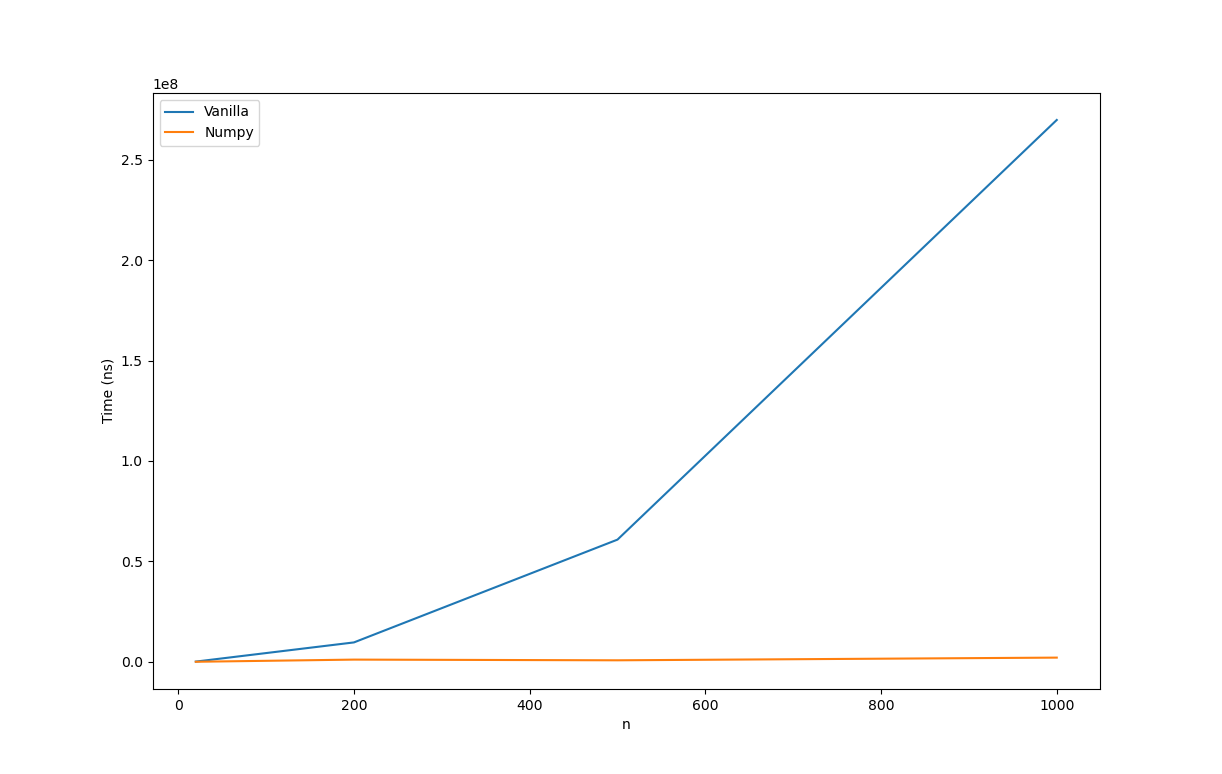
\includegraphics[width=1\textwidth]{../Figure_1.png}

            \textbf{Reason:} \\
            For vanilla python, we are manually looping through the list and vectors to do matrix operations on
            the python level, but NumPy uses optimized low level C precompiles to do the matrix operations. The optimized memory
            access pattern allowed the running time for NumPy solution to grow much slower than the vanilla python solution.
        \end{answer}
     \end{part}

\end{question}

%%%%%%%%%%%%%%%%%%%%%%%% Task 9 %%%%%%%%%%%%%%%%%%%%%%%%
\begin{question}{A10. (4 points)} 
    \begin{part}
        \begin{answer}
            \textbf{n = 40000}
         \end{answer}
     \end{part}

     \begin{part}
        \begin{answer}
           \textbf{How does the empirical CDF change with $k$?}\\
            As $k$ increases, the empirical CDF becomes more and more similar (converges) to the true CDF. \\
         \end{answer}
     \end{part}

     \begin{answer}
        \textbf{Plot of $\widehat{F}_n(x) \in [-3, 3]$:} \\
        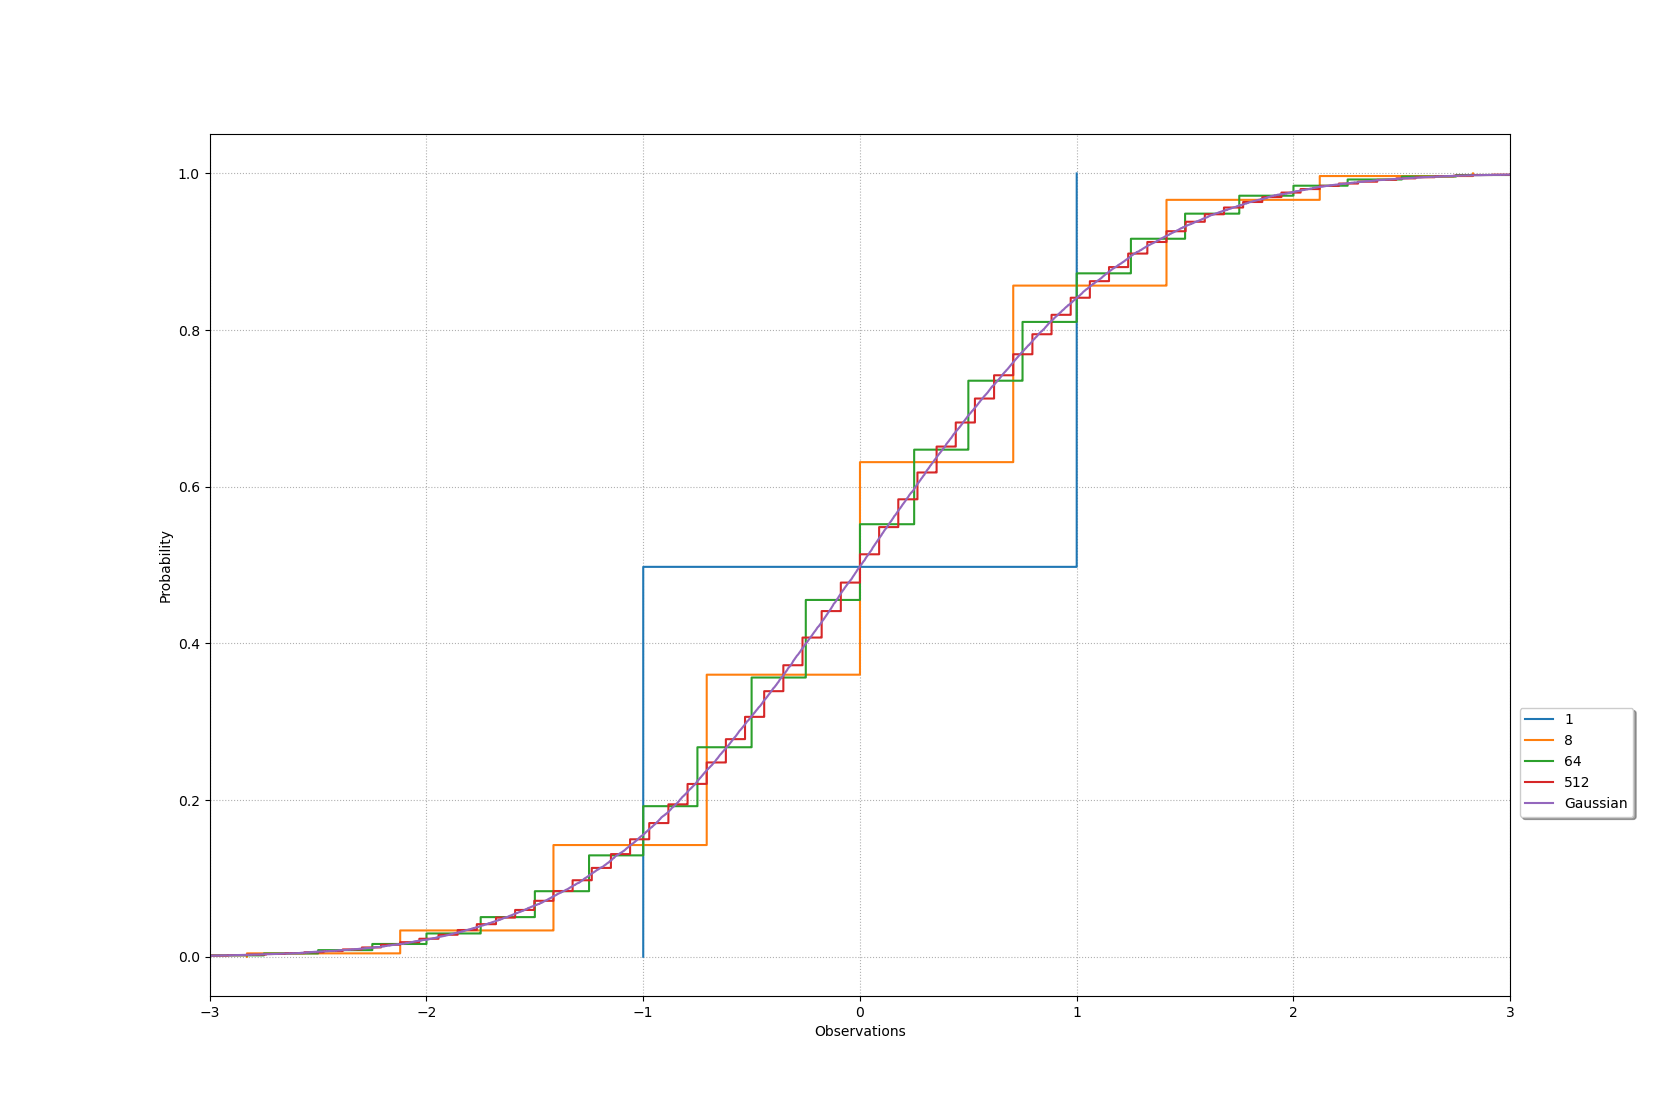
\includegraphics[width=1\textwidth]{../Figure_2.png}
     \end{answer}

\end{question}
\end{document}

